\newcommand{\figureSmallLCDShematics}[1]{
  \def\lang{\detokenize{#1}}
  \def\langRu{\detokenize{ru}}
  \def\langEn{\detokenize{en}}
  \def\figureCaption{XXX: No translation.}
  \ifx \lang\langRu
  \def\figureCaption{
    Схематическое изображение дисплея 16x2 (16 столбцов, 2 строки.)
  }
  \fi
  \ifx \lang\langEn
  \def\figureCaption{
    A schematic representation of an 16x2 LCD (16 columns, 2 rows.)
  }
  \fi
  \begin{figure}[ht]
    \centering
    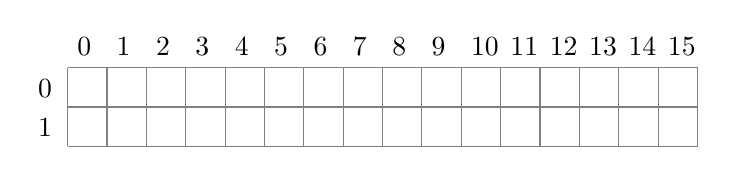
\begin{tikzpicture}
      \draw[gray, step=0.5] (0, 0) grid (8, 1);
      \foreach [count=\i from 0] \x in {0.0, 0.5, 1.0, ..., 7.5} {
        \draw (\x, 1.5) node[anchor=north west] {\i};
      }
      \foreach [count=\i from 0] \y in {0.5, 0.0} {
        \draw (-0.5, \y) node[anchor=south west] {\i};
      }
    \end{tikzpicture}
    \caption{\figureCaption}
    \label{fig:lcd-16x2-schematics}
  \end{figure}
}
